\chapter{微流控线虫芯片的设计及硬件平台的搭建}
\section{引言}
	在传统的线虫毒理实验过程中,通过人工的方式在96孔板上配置不同浓度的化合物。
	然后将线虫暴露在不同浓度的化合物下,观察并记录线虫在不同浓度化合物下
	的变化。这种人工操作的方式不仅存在样品消耗大、通量低和操作繁琐等缺点, 
	而且也不利于观察。本章设计了两款微流控芯片分别用于线虫的急性毒性实验
	和需要对线虫长期培养的慢性毒性实验。为了实现对这两款芯片的进样控制和阀门控制,
	本课题组开发了自动化阀门控制系统。同时用多线程的方法优化了线虫视频采集的速度,
	为后续的线虫特征提取提供了视频数据。
\section{实验材料与仪器}
	
	\begin{table}[htbp]
	\centering
	\bicaption
    {实验试剂与耗材}
    {Experimental reagents and consumables}
	\begin{tabular}{p{150pt}p{230pt}}
	\toprule
		光刻胶SU-83050 & 美国Microchem公司\\
		光刻胶AZ4903 & 德国Merck Performance Materials公司\\
		聚二甲基硅氧烷PDMS( polydimethylsiloxame, RTV 615) &美国 Momentive Performance Materials 公司\\
		氟化液FC-40 & 北京伊诺凯科技有限公司\\
		FA1004分析电子天平 & 上海良平仪器仪表有限公司\\
		RC8型匀胶机 & 美国 Karl Suss公司\\
		DZF-6020型真空干燥箱& 上海新苗医疗器械制造有限公司\\
		ZXZ-2型旋片式真空泵 & 浙江谭氏真空设备有限公司\\
		SMZ-168型体式显微镜& 中国麦克奥迪公司 \\
		NMC反应离子式深硅刻蚀系统 & 北京北方微电子公司\\
		IX71型倒置荧光显微镜 & 日本Olympus公司\\
		DP73型CCD & 日本Olympus公司\\
	\bottomrule
	\end{tabular}
	\end{table}	
\section{用于线虫急性毒理实验的梯度稀释芯片设计及制作}
\subsection{用于线虫急性毒理实验的梯度稀释芯片设计}
\label{arch-design}
本文首先设计了一款用于急性毒理实验的双层微流控芯片,用于快速形成化合物梯度浓度,
并与线虫进行反应,以观察不同化合物浓度对线虫生长发育的影响。
其制作工艺采用了基于Quake的双层阀门工艺,Quake阀门原理如图\ref{fig:chap2:path}所示,
当向阀门层施加一定的气压时,PDMS模会在气压的作用下被顶起从而压迫上层的流道,使
流道关闭,下层的阀门层起到了阀门的作用。
	\begin{figure}[htbp]
	  \centering
	  \includegraphics[width=10cm]{figure/chap2/path.jpg}
	  \bicaption
		{Quake阀门原理示意图}
		{Schematic diagram of Quake valve}
	  \label{fig:chap2:path}
	\end{figure}
\begin{figure}[htbp]
	  \centering
	  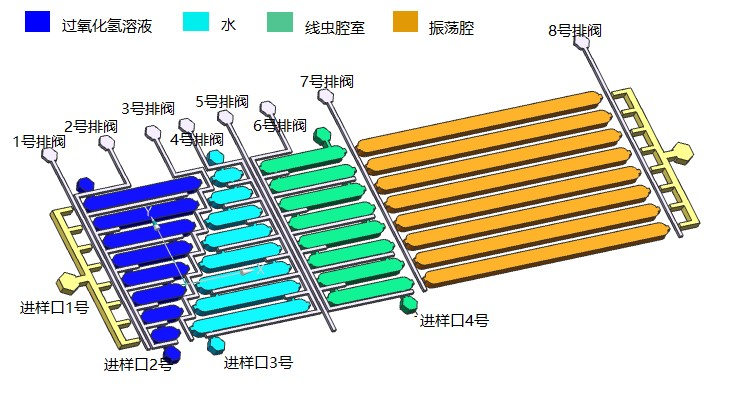
\includegraphics[width=13cm]{figure/chap2/chip-arch.png}
	  \bicaption
		{线性梯度稀释芯片结构}
		{Structure of Linear gradient dilution chip}
	  \label{fig:chap2:chip-arch}
	\end{figure}
	
图\ref{fig:chap2:chip-arch}为线性梯度稀释芯片的结构示意图,
该芯片由两层PDMS组成,上层为流道层,下层为阀门层。
片上有4个进样口、4个出样口和8个排阀。8个排阀控制每列之间的隔绝和连通以及
每列9个腔室之间的隔绝和连通。
4列腔室之间的隔绝与连通由3、5、7号排阀控制,而2、4、6号排阀分别控制1、2、3列里
9个腔室之间的隔绝与连通,整个梯度稀释芯片由8个排阀分成$9\times4$个独立的腔室。
4列腔室中第一列9个腔室的长度依次线性递减,第二列9个腔室的长度依次线性增加,前两列腔室的长度总和为2mm (两腔室长度的比例从上到下依次为$9:1,8:2,\dots,1:9$)。
第三列和第四列腔室的长度保持恒定分别为1mm和3mm。所有腔室的宽度和高度分别为200$\mu$m和80$\mu$m。

\subsection{芯片模具加工工艺}
\subsubsection{阀门层模具制作}
	
	\begin{enumerate}[label={(\arabic*)},font={\color{black!50!black}\bfseries}]
	\item 按照\ref{arch-design}小节的结构设计使用AutoCAD绘图软件绘制阀门层的结构图案并制作掩模版。
	\item 在涂胶之前,需先将3英寸的单抛硅片放在180$^\circ C$的烘箱中2小时,然后用氧等离子体去胶机处理60秒。
	\item 旋涂光刻胶AZ4903并用200rpm的转速预转8秒,然后再用1000rpm的转速甩胶25秒得到22um厚的胶。
	\item 将硅片放入烘箱中,逐渐升温至$50^\circ C$,30分钟后再将温度升高至$90^\circ C$,90分钟后再将其取出。
	\item 经过紫外曝光后再显影。
	\item 为了去除硅片表面的水汽,将其放入$80^\circ C$的烘箱中1小时,最后使用甲基三氯硅烷处理硅片表面5分钟。
	\end{enumerate}
	
\subsubsection{流道层模具制作}
	由于本文中芯片的管道和腔室的高度被设计成不同的尺寸,且腔室的高度要比管道的高度要高,
	所以需要经过两次光刻才能完成流道层模具的制作,第一次光刻采用正胶制作管道结构,第二次光刻采用负胶制作腔室结构。
	\begin{enumerate}[label={(\arabic*)},font={\color{black!50!black}\bfseries}]
	\item 使用AutoCAD绘图软件分别绘制芯片管道和芯片腔室的结构并打印制作掩模。
	\item 在涂胶之前,需先将3英寸的单抛硅片放在180$^\circ C$的烘箱中2小时,然后用氧等离子体去胶机处理60秒。
	\item 旋涂光刻胶AZ4903并用200rpm的转速预转8秒,然后再用1000rpm的转速旋涂25秒得到22um厚的胶。
	\item 将硅片放入烘箱中,逐渐升温至$50^\circ C$,30分钟后再将温度升高至$90^\circ C$,90分钟后再将其取出。
	\item 经过紫外曝光后再显影。
	\item 将硅片放在热板上分别升高温度分别在$65^\circ C$、$95^\circ C$、$120^\circ C$和$190^\circ C$分别停留
	5min、5min、40min和60min。这个步骤是正胶回流使管道的截面形成弧形结构,
		而弧形结构才能保证阀门层施加压力时候完全截断管道。
	\item 旋涂负胶SU-8 3050并用500rpm的转速预转8秒,然后再用1500rpm的转速旋涂30秒得到80um厚的胶。
	\item 将硅片放在$95^\circ C$的烘箱中恒温40min。
	\item 经紫外曝光后将硅片放入$95^\circ C$的烘箱中恒温60min。
	\item 用对应的显影液对硅片显影,并用异丙酮溶液漂洗,以除去残留的显影液和试剂残留并用氮气将硅片吹干。
	\item 为了除去水汽,将硅片放入$80^\circ C$的烘箱中恒温60min,再用甲基硅氧烷处理5min。
	\end{enumerate}
\subsection{双层微流控芯片的制作}
	制作好芯片模具后,就可以利用芯片模具进行微流控芯片的制作,下面将介绍双层微流控芯片的制作流程。经过以下流程
	最终完成的芯片其实物图如图\ref{fig:chap2:chip-fabric}所示,为了更好地显示芯片结构,芯片的四列腔室
	都被打入不同颜色的染料。
	\begin{enumerate}[label={(\arabic*)},font={\color{black!50!black}\bfseries}]
	\item 将流道层硅片的背面用胶粘在一次性培养皿的底部,起到一个固定的作用。
	\item 配制PDMS:按照20:1的比例,取20克RTV 615(A液)和1克固化剂(B液)混合搅拌均与,按照5:1的比例,
	取20克RTV 615(A液)和4克固化剂(B液)混合搅拌均匀,并将两种比例的混合液放入真空皿中抽真空以排出液体中的气泡,
	不断地抽气放气直到液体呈现澄清状。
	\item 将5:1的PDMS混合液倒入流道层培养皿中,PDMS混合液的厚度大约5mm左右。
	\item 将阀门层硅片放在甩胶机吸盘的中心位置,并用真空吸住硅片使其固定,将20:1的PDMS混合液倾倒在硅片上,
	用400rpm的转速预转20秒后再用1800rpm的转速转60秒即可得到厚约40um的PDMS层。
	\item 将阀门层模具和流道层模具一起放入$80^\circ C$的烘箱中恒温30min。
	\item 用手术刀将培养皿中的PDMS层沿着硅片的边沿切下并取出。再用铲刀沿着芯片上的图案将其切成长方形。
	\item 在显微镜下将上一步切下的流道层芯片与阀门层对准并粘合在一起。
	\item 将其放入$75^\circ C$的烘箱中恒温5个小时进行高温键合,然后将其取出放在无尘纸上进行常温冷却。
	\item 再用打孔器将芯片的进样口、出样口和阀门入口位置打孔。
	\item 将芯片和干净的玻璃片一起放入氧等离子体去胶机中处理40秒后,将芯片和玻璃贴合在一起并放入$80^\circ C$的烘箱中
	恒温2小时。
	\end{enumerate}
	\begin{figure}[htbp]
	  \centering
	  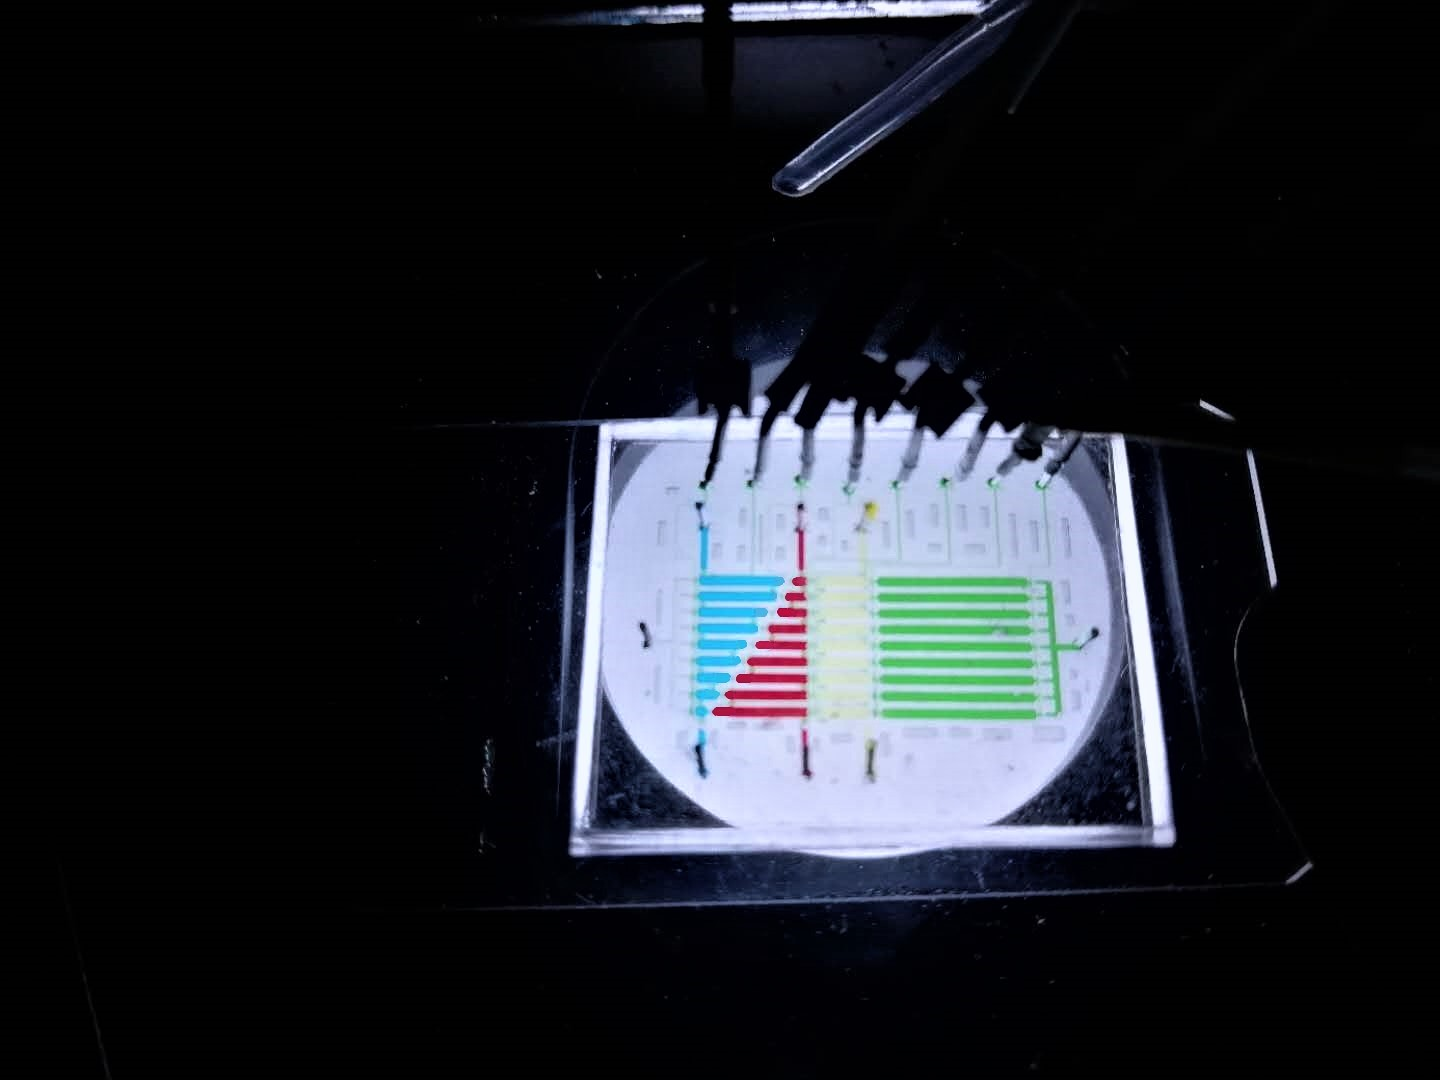
\includegraphics[width=9cm]{figure/chap2/fabric-chip.jpg}
	  \bicaption
		{线性梯度稀释芯片实物图}
		{fabricated linear gradient dilution chip}
	  \label{fig:chap2:chip-fabric}
	\end{figure}
\subsection{染料与荧光实验}
	梯度稀释是生物化学领域常用的技术,在微流控芯片上研究梯度形成的研究也较多,
	如经典的“圣诞树”结构\cite{Dertinger2001Generation,Jeon2000Generation},
	但其存在样品消耗大以及需要精确的流阻设计和流速调节等问题。
	本文提出一种基于振荡原理的集成高通量阀门的梯度芯片结构,可以快速形成多个浓度梯度。
	芯片管道中不同液体的混合使用了本课题组提出的只需一个压力源的基于流体振荡的混合方式\cite{cheng2018simple}。
	振荡的时候需要在管道的一端构造一个封闭的空腔环境。
	当需要将前两列腔室中的液体混合时,可以将第三列腔室作为储气腔,
	将7号排阀关闭即可形成封闭的储气腔;
	当需要将前三列腔室中的液体混合时,可以将第四列腔室作为储气腔。

	为观察振荡混合的效果以及验证梯度形成的准确性,
	本文使用了红色染料及荧光试剂对芯片进行测试。如图\ref{fig:before}所示,
	分别向第一列腔室和第二列腔室中打入红色染料和水,将腔室中的空气全部排出
	,使液体充满整个腔室。
	将第三列腔室作为振荡腔,在1号进样口施加一个周期为250ms压力值为0.05Mpa的气压,
	经过7分钟的振荡,染料和水完全混合后的效果如图\ref{fig:after}所示。
	从图中可以看出红色染料已经充分混合均匀,且从最上面的腔室到最下面的腔室
	红色染料的颜色依次变淡。
	在不加振荡的情况下,两列腔室中的液体以自由扩散方式完成以上混合
	需要2~3个小时。可以看出,基于振荡的混合方式对快速形成浓度梯度有较好的效果,
	能够显著加快不同液体的混合速率。
	
	为了验证梯度形成的准确性,本文将100$\mu$M的异硫氰酸荧光素(FITC)作为待稀释样品打入第一列腔室,
	将磷酸缓冲液(PBS)作为稀释剂打入第二列腔室,在相同的振荡参数下完成振荡混合,
	最终得到$10\mu M,20\mu M,\cdots,90\mu M$的线性浓度梯度。使用奥林巴斯荧光倒置显微镜(IX-73)和
	DP73型CCD拍摄每个腔室中的荧光染料图像,用Image J图像处理软件将图像转成8位灰度图
	并读取光强。图\ref{fig:chap2:fluence}为各个腔室中FITC浓度与荧光强度之间的关系,
	图中蓝色的线表示线性拟合的结果,可以看出拟合结果的线性度较好。
	为了验证线虫经过振荡混合后不会留下不良后果,
	本文将线虫溶液打入第三列腔室,并在以上振荡参数下完成振荡,
	观察2个小时发现线虫的摆动频率与没有经过振荡的线虫相比没有明显差异。通过以上实验证明了
	梯度稀释芯片设计的合理性,该芯片可以在较短的时间内形成准确的浓度梯度,
	可以用于研究线性浓度梯度的化合物对秀丽隐杆线虫的影响。

	\begin{figure}[!thp]
	\centering
	  \begin{subfigure}{0.45\textwidth}
		\centering
		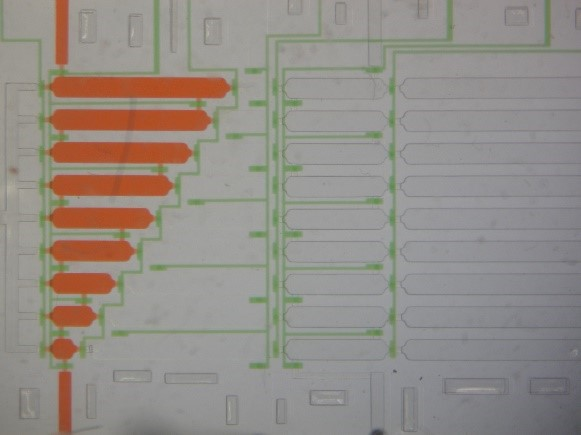
\includegraphics[width=1\linewidth]{figure/chap2/before.jpg}
		\caption{振荡前的芯片图 }
		\label{fig:before}   
	  \end{subfigure}
		\hspace{1em}
	  \begin{subfigure}{0.45\textwidth}
		\centering
		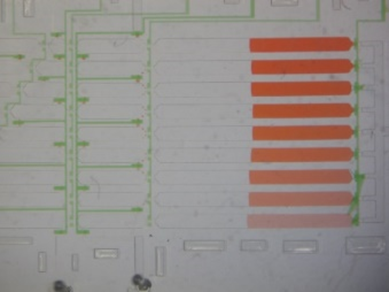
\includegraphics[width=1\linewidth]{figure/chap2/after.png}
		\caption{振荡结束后的芯片图}
		\label{fig:after}
	  \end{subfigure}
	  \bicaption{振荡前后各个腔室染料颜色的变化}
	  {Color change of dyes in each chamber before and after oscillation}
	  \label{fig:oscillation}
	\end{figure}

	\begin{figure}[htbp]
	  \centering
	  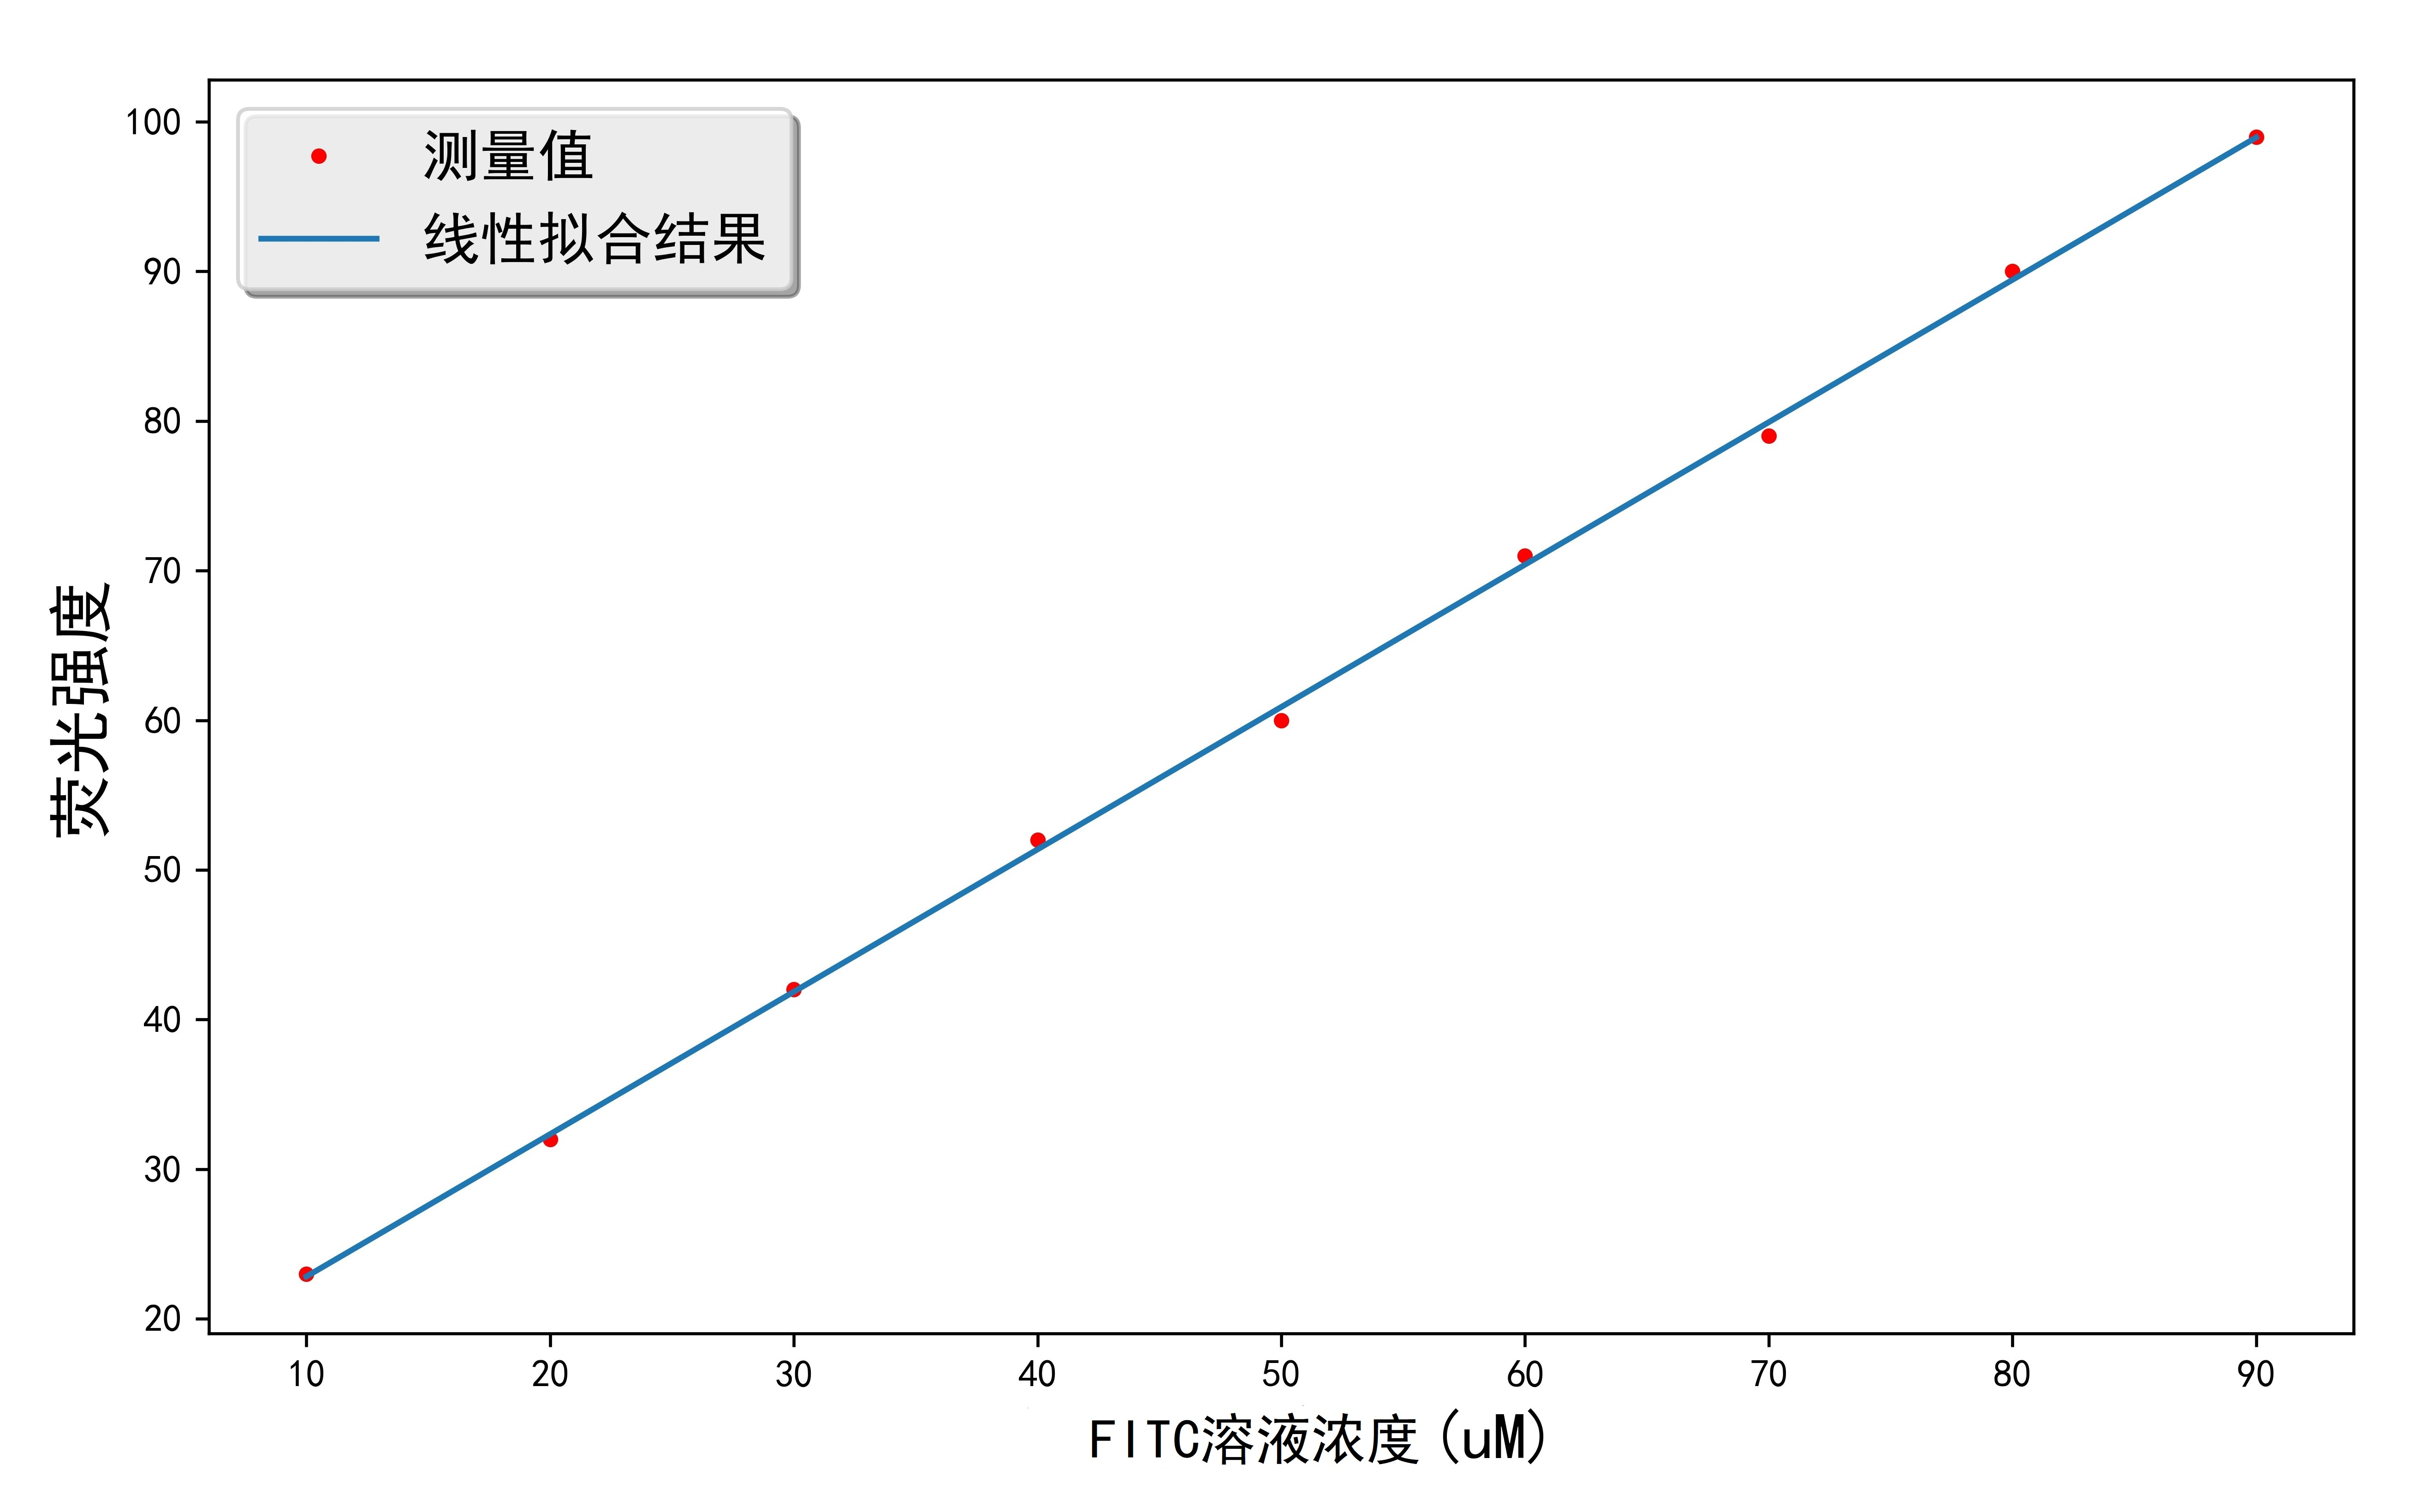
\includegraphics[width=11cm]{figure/chap2/fluence.jpg}
	  \bicaption
		{各腔室不同浓度FITC溶液荧光强度变化}
		{Fluorescence intensity changes with different concentrations of FITC solution in each chamber}
	  \label{fig:chap2:fluence}
	\end{figure}
\section{用于线虫长期培养的慢性毒理芯片的设计及制作}
\subsection{用于线虫长期培养的慢性毒理芯片设计}
\label{subsec:chipdesign}
	\begin{figure}[!b]
	  \centering
	  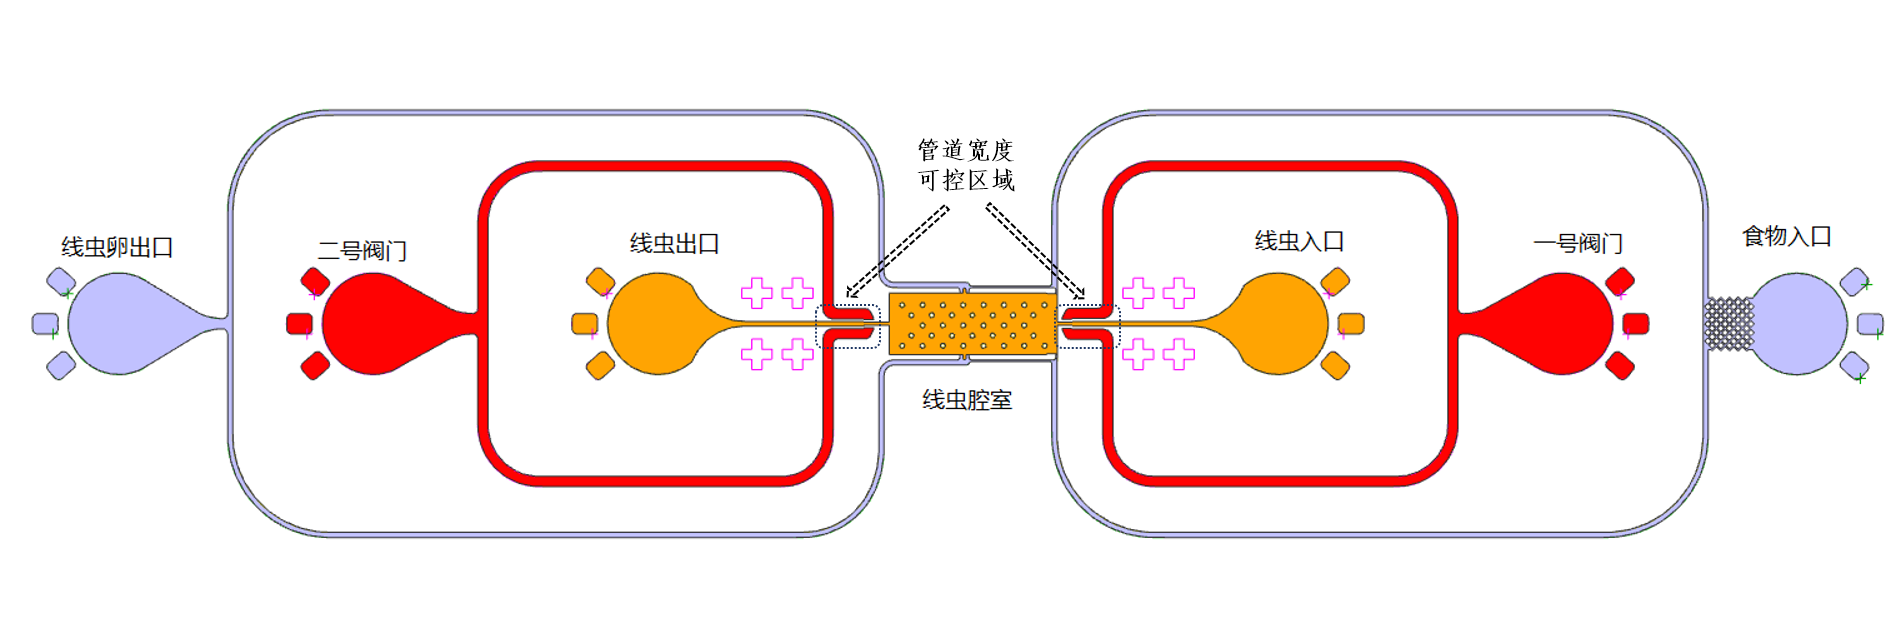
\includegraphics[width=14cm]{figure/chap2/arch-chip.png}
	  \bicaption
		{单层阀门线虫培养芯片}
		{Single layer lateral valve chip for  worm culture}
	  \label{fig:chap2:singlelayer}
	\end{figure}
	本文在\ref{arch-design}小节设计的用于急性毒理实验的双层芯片制作工艺较复杂,且没有设计食物
	供应的通道,不适合应用在需要对线虫进行长期培养观察的慢性毒性实验中。
	本小节将介绍另一种带侧向阀门的单层毒理芯片,该芯片不仅制作工艺简单而且还可用于线虫的长期培养,
    如图\ref{fig:chap2:singlelayer}所示是带侧向阀门的单层毒理芯片设计图。
	图中可以看出芯片可以分成三个部分,本文
	分别用三种不同的颜色表示。中间黄色的区域为线虫培养腔室。
	由于腔室的面积比较大且PDMS是柔性材料,
	为了防止腔室塌陷,腔室里放置了微柱,图中线虫入口和线虫出口分别表示线虫的进样口和出样口
	。红色管道为本文设计的侧向
	阀门,通过对阀门施加气压可以控制线虫培养腔室两端通道宽度的大小。这种侧向阀门的设计可以控制腔室中
	线虫的进入和排出,相当于一个夹子的作用,从而可以控制腔室中线虫的数量。
	最外层的设计为线虫提供食物和虫卵的排出。右边为食物的
	入口,其中的网状结构可以过滤掉食物中的小碎片。虫卵会通过线虫腔室的侧向通道被排出,
	从而可以防止不同代的
	线虫出现在同一个腔室,可以针对同一代的线虫进行实验观察。

\subsection{单层阀门芯片模具的制作}
	下面开始介绍单层阀门芯片模具的制作工艺流程。
	\begin{enumerate}[label={(\arabic*)},font={\color{black!50!black}\bfseries}]
	\item 根据芯片结构的尺寸设计运用AutoCAD绘图软件绘制芯片的二维结构并制作掩模版。
	\item 为了使光刻胶和硅片更容易结合,必须充分去除硅片的水分。将单面抛光的3寸硅片放进
	$180^\circ C$烘箱中恒温$2\sim3$个小时。
	\item 将硅片从烘箱中取出,待其恢复到室温后,用氮气将硅片表面的杂质吹掉使硅片表面保持干净。
	用光刻胶AZ-4903倒在硅片的中心出,使其自然铺开慢慢覆盖硅片表面。然后5000rpm的转速旋涂30s得到胶层厚度
	大约为1um。
	\item 为了去除光刻胶中的有机溶剂并使光刻胶固定需要经过前烘,将涂有光刻胶的硅片放入烘箱中。将烘箱的温度
	缓慢升至$65^\circ C$,恒温30min。然后继续将温度升至$90^\circ C$,再恒温30min,最后慢慢将烘箱温度降至
	室温。
	\item 将硅片放入光刻机中,曝光前,先打开光刻机汞灯预热10min分钟。将掩模版放在硅片上面并中心对齐,根据
	光刻机的厚度调整好曝光时间,经过曝光处理后,将可掩模上的图案转移到光刻胶上。
	\item 将经过曝光处理的硅片放入烘箱中逐渐升温至$65^\circ C$并恒温15min,然后再逐渐升温至$95^\circ C$
	恒温40min,最后慢慢将温度降到室温。
	\item 经过后烘步骤,再用对应的显影液对硅片进行显影,得到清晰的图形后再用氮气将硅片表面吹干。
	\item 将硅片放入深硅刻蚀机中,进行干法刻蚀。光刻胶覆盖的区域将不会被刻蚀,从而可以将掩模板上的芯片
	图案转移到硅片表面。注意根据腔室的高度,控制好刻蚀的厚度。
	\item 为了使PDMS芯片的制作过程中,PDMS层容易从模具上揭下来,需要对硅片表面进行硅烷化处理。
	将硅片放入一次性的培养皿中,在硅片旁的滤纸上滴一滴硅烷化试剂,通过蒸发沉淀的方式完成硅烷化处理。
	\end{enumerate}
		\begin{figure}[!tbp]
	  \centering
	  \includegraphics[width=12cm]{figure/chap2/fabric-chip2.jpg}
	  \bicaption
		{单层侧向阀门线虫培养芯片实物图}
		{Fabricated single layer lateral valve chip for worm culture}
	  \label{fig:chap2:fabricsinglelayer}
	\end{figure}
\subsection{单层阀门芯片的制作}
	将 PDMS 浇筑在芯片的模具上待其固化,即可完成单层侧向阀门芯片的制作,
  通过以下工艺流程最终制作完成的芯片如图\ref{fig:chap2:fabricsinglelayer}所示。

	\begin{enumerate}[label={(\arabic*)},font={\color{black!50!black}\bfseries}]
	\item 将硅片模具固定在一次性的培养皿的底部。
	\item 配置PDMS混合液:按照10:1的比例,取20克的PDMS(Sylgard 184)A液和2克的固化剂(B液)混合搅拌均匀,
	并将两种比例的混合液放入真空皿中抽真空以排出液体中的气泡,不断地抽气放气直到液体呈现澄清状。
	\item 将PDMS浇筑在放有硅片模具的培养皿中,浇筑厚度约为5mm,重新放回真空皿中抽出芯片表面的气泡。
	\item 将培养皿放入$75^\circ C$的烘箱中恒温一个小时使PDMS得以固化。
	\item 从烘箱中取出芯片模具,待其自然冷却,用手术刀将PDMS层从模具上揭下来。按照芯片上的图案用PDMS切成方形,
	并在所有进口、出口处打孔。
	\item 将芯片和干净的玻璃片一起放入氧等离子体去胶机中处理40 秒后,将芯
片和玻璃贴合在一起并放入$80^\circ C$的烘箱中恒温2小时,加强键合效果。
	\end{enumerate}
\subsection{慢性毒理芯片的侧向阀门测试}
	为了测试侧向阀门的设计可以控制腔室两端管道的宽度,
	本文测试了不同压力下管道宽度的变化。为了便于视觉
	观察,我们向阀门通道注入了红色的染料。
	图\ref{fig:chap1:width}表示向阀门施加不同压力的情况下腔室两端通道的
	宽度变化。从图中可以看出在0.3Mpa的压力下,通道的宽度明显变窄了。
	该测试结果表明这种侧向阀门的设计可以改变通道的宽度,
	通过控制腔室两端通道的宽度可以控制
	线虫的进入或排出。
		\begin{figure}[!htp]
	  \centering
	  \begin{subfigure}{0.45\textwidth}
		\centering
		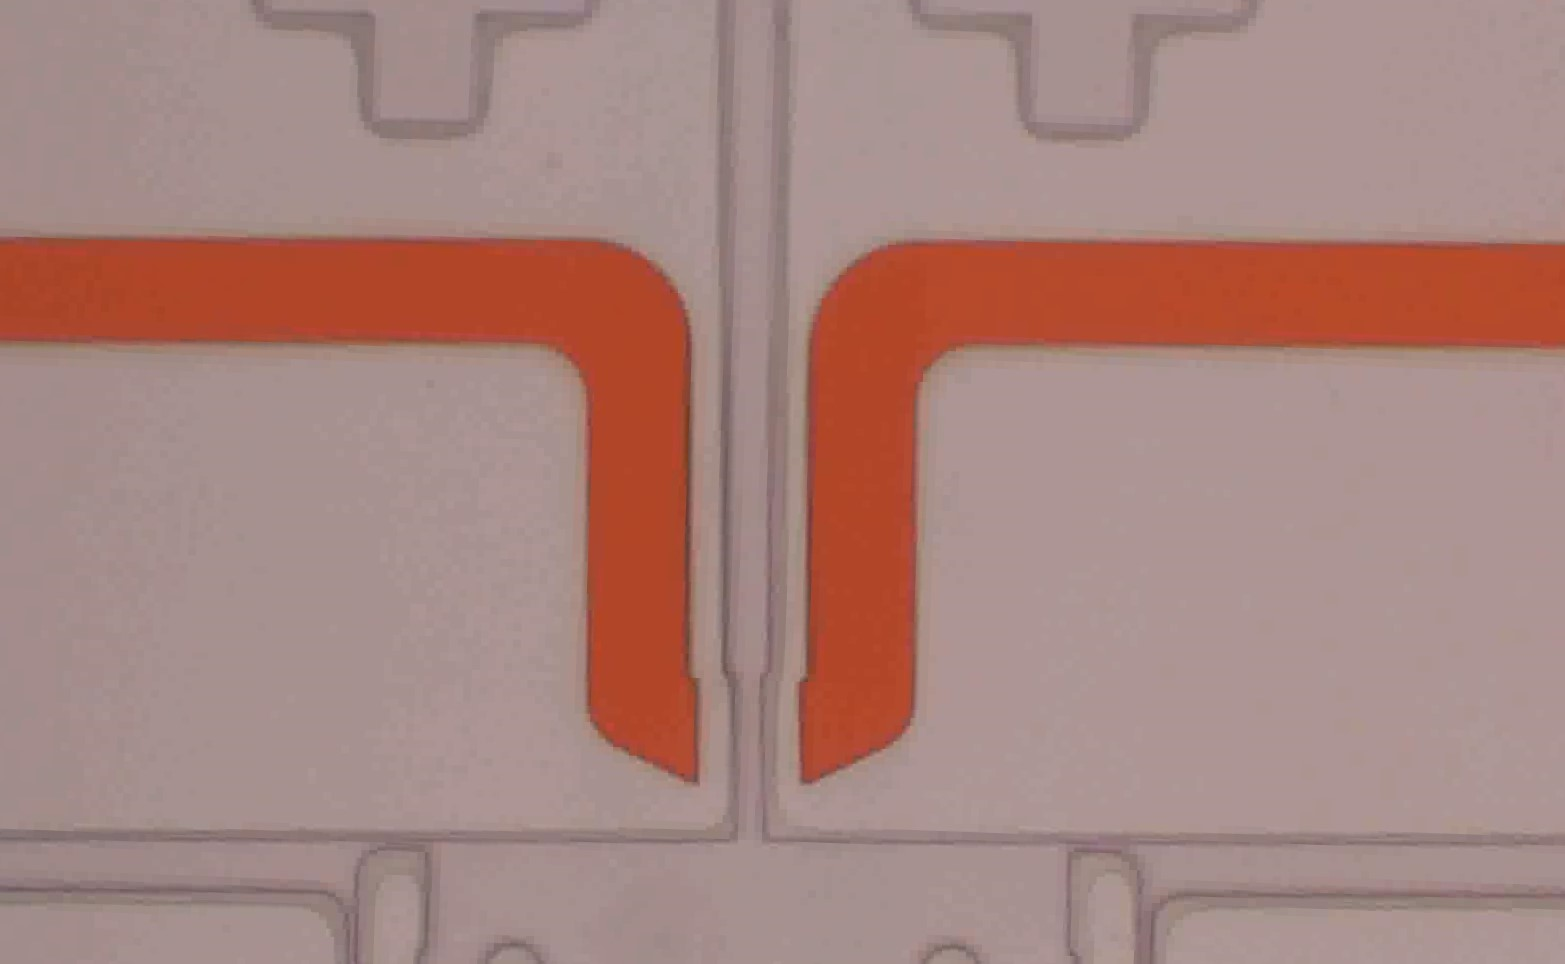
\includegraphics[width=1\linewidth]{figure/chap1/singlelayertest1.jpg}
		\caption{没有对阀门施加压力的情况下通道宽度}
		\label{fig:before1}   
	  \end{subfigure}
		\hspace{1em}
	  \begin{subfigure}{0.45\textwidth}
		\centering
		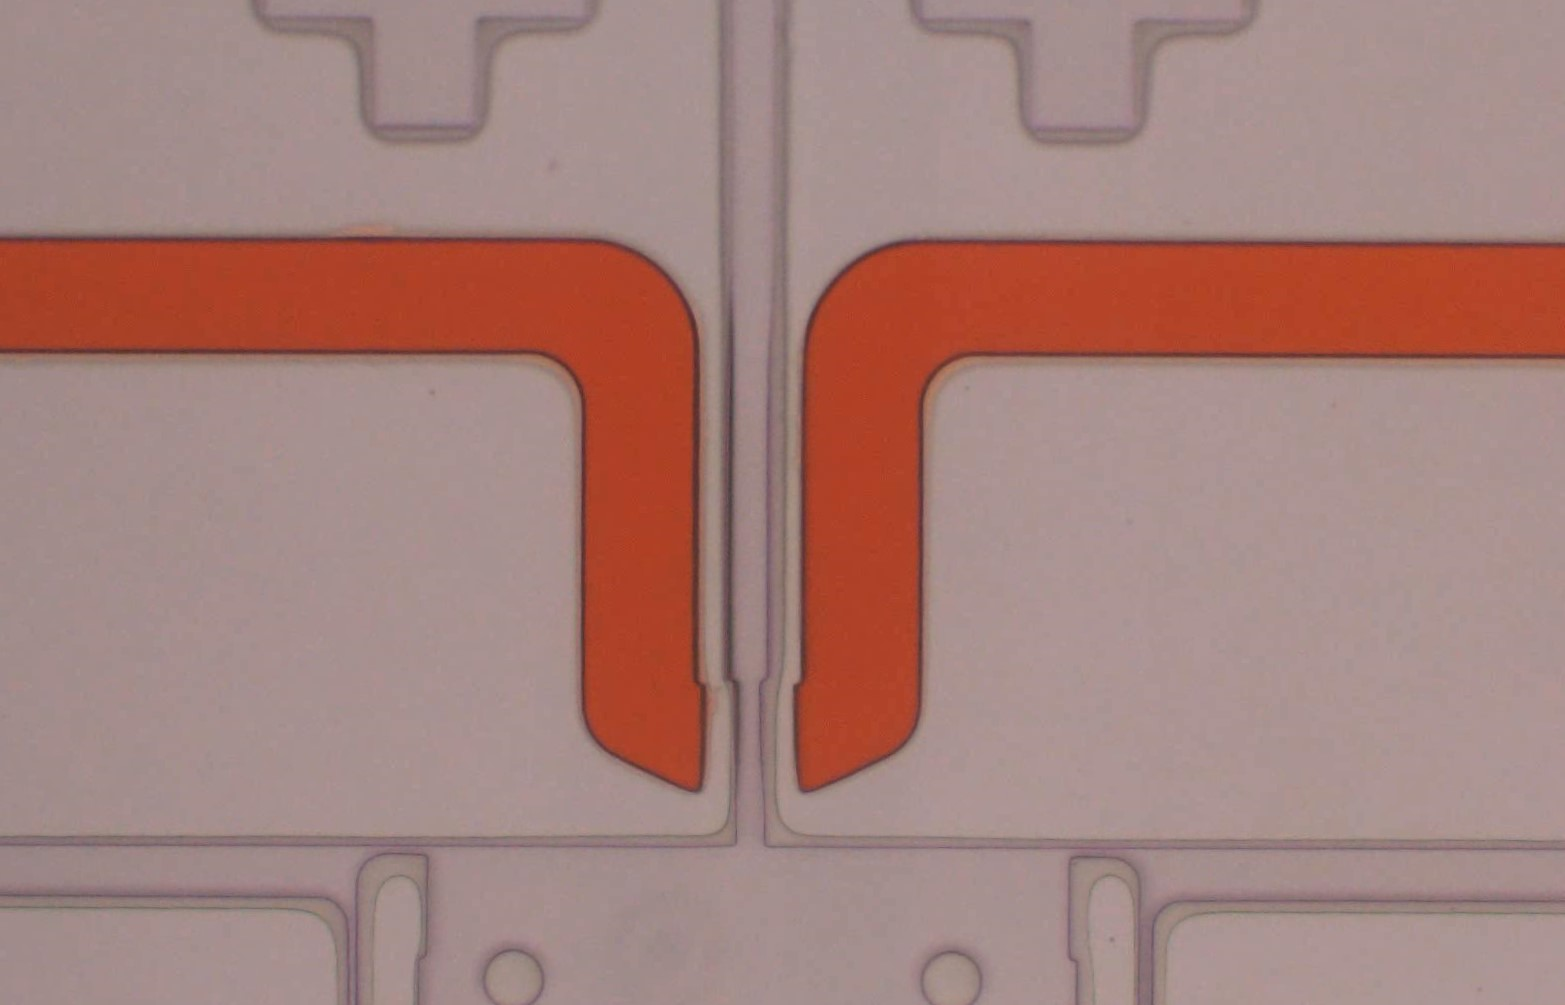
\includegraphics[width=1\linewidth]{figure/chap1/singlelayertest2.jpg}
		\caption{向阀门施加0.3Mpa压力下的通道宽度}
		\label{fig:after1}
	  \end{subfigure}
	  \bicaption{不同压力下通道宽度的变换}{Transform of channel width under different pressure}
	  \label{fig:chap1:width}
	\end{figure}
	\begin{figure}[!htp]
    \centering
    \begin{tikzpicture}[node distance=2.5cm,auto]
	\tikzstyle{process} = [rectangle,rounded corners,thick,minimum width = 3cm,text width=3cm,inner sep=2pt,minimum height =1.7cm, text centered, draw = black]
    \node (pc) [process] {手机/平板};
    \node (mcu) [process, below of=pc] {微控制器及运算放大器};
    \node (valves) [process, below of=mcu] {电磁阀};
    \node (pump) [process, right of=valves,node distance=4cm] {气泵};
    \node (chip) [process, left of=valves,node distance=4cm] {微流控芯片};
    %连接具体形状
    \draw [arrow](pc) -- (mcu);
    \draw [arrow](mcu) -- (valves);
    \draw [arrow](valves) -- (chip);
    \draw [arrow](pump) -- (valves);
	\end{tikzpicture}
    \bicaption{自动化阀门控制系统}{Automated valve control system}
    \label{fig:flow_chart}
	\end{figure}
\section{阀门控制系统搭建}
	目前,双层的微流控芯片一般由下层的阀门层和上层的流道层组成。阀门层的PDMS薄膜通常很薄,当向气阀通道施加一定的
	气压(大约30psig),阀门层的薄膜会向上顶起。由于上层的流道和下层的气阀通道是上下交叉的,通过控制向气阀通道施加
	气压,便可以控制上层流道的通断。另一方面,线虫的压力进样和芯片的振荡都需要对进样口进行气压控制。基于以上需求
	,本课题组开发了自动化阀门控制系统,图\ref{fig:flow_chart}为该系统的连接示意图。整个系统由五个模块构成,
	我们采用了750W-18L小型空压机作为气泵模块为整个系统提供气压输出,将Arduino作为微控制器控制电磁阀的输出。
	Arduino由运行在手机/平板上的上位机程序控制。通过该系统可以实现对线虫微流控芯片阀门和进样的控制。
	图\ref{fig:chap2:valve}为多路阀门控制仪器的实物图,图\ref{fig:chap2:controlpanel}
	为多路阀门控制仪器的控制界面。
	\begin{figure}[!ht]
	  \centering
	  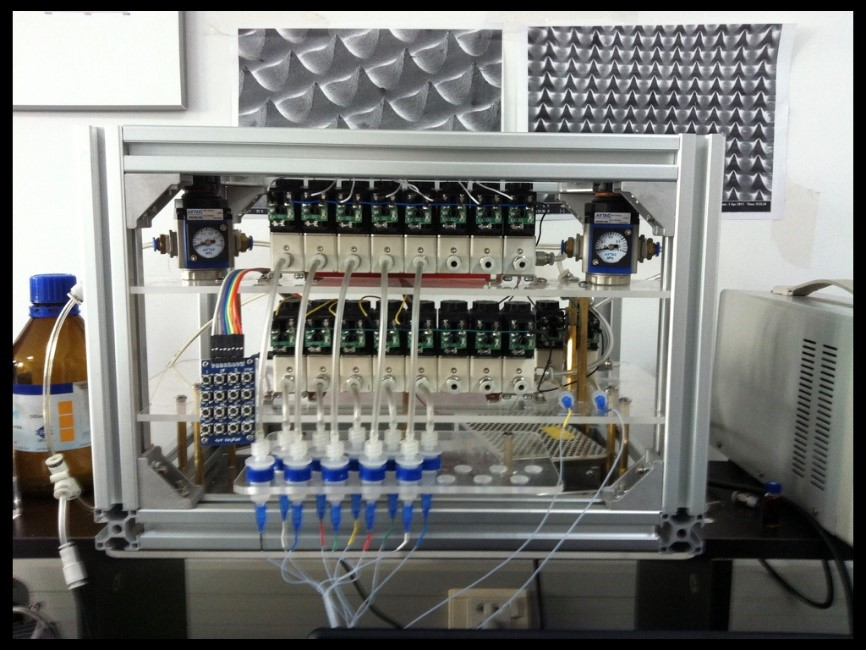
\includegraphics[width=10cm]{figure/chap2/controlsys.jpg}
	  \bicaption
		{多路阀门控制仪器}%和电脑控制仪器界面and user interface of the control instrument on the computer
		{Valve control equipment }
	  \label{fig:chap2:valve}
	\end{figure}
	\begin{figure}[!ht]
	  \centering
	  \includegraphics[width=10cm]{figure/chap2/controlpanel.jpg}
	  \bicaption
		{手机/平板控制仪器界面}%和电脑控制仪器界面and user interface of the control instrument on the computer
		{User interface of the control instrument on phone or pad }
	  \label{fig:chap2:controlpanel}
	\end{figure}
\section{线虫视频采集帧率的优化}
	线虫视频的高速采集对线虫摆动频率的估计是至关重要的一步。根据采样定理,采集的视频帧率至少是线虫摆动频率的两倍。
	除了采样频率的要求外,视频的分辨率等因素同样影响后续线虫图像处理的难度。基于以上考虑,本文选取鑫图公司的DigiRetina 16
	 COMS相机作为线虫视频的采集模块。其可以通过USB3.0高速传输接口与电脑进行高速图像数据传输,同时该相机在放大倍率20
	 倍以下的显微成像中,也可以获得分辨率优异的显微图像,另外其内置两个FPGA双核处理器分别用于高清图像处理和
	 图像输出控制。该相机较好满足了本文对线虫视频采集模块的要求。为了提高视频采集的帧率,
	 本文基于该相机的SDK,开发基于多线程
	 的视频采集程序。
	 
	相机的SDK 以动态链接库(Dynamic Link Library, DLL)的形式提供,而本文采用 python 作为开发语言进行高速视频采集程序的设计,
	因此不能直接调用 SDK。ctypes 是python 的第三方库,它提供了与 C 语言兼容的数据类型。
	通过这个第三方库,使 python 具有调用动态链接库的能力,因此可以通过python对相机进行操作。
	视频的写入通过opencv提供的VideoWriter类实现。在相机SDK提供的API函数中有两个重要的与图像获取相关
	的函数分别是TUCAM\_Buf\_WaitForFrame 函数和TUCAM\_Buf\_CopyFrame函数。
	TUCAM\_Buf\_WaitForFrame函数用于等待数据捕获完成,这个函数属于阻塞函数。
	TUCAM\_Buf\_CopyFrame 函数用于将捕获的图像数据传输到电脑内存中,
	图像数据的格式需要在相机初始后设置。本文将相机的帧格式设置为彩色RGB模式,
	图像像素在内存中按照从左到右从上到下的方式连续存储。且每一个像素有RGB
	三个颜色通道,每个颜色通道都用一个字节存储。为了将图像数据转化为numpy数组,
	方便python访问,本文使用 C 函数库中的 memcpy 内存拷贝函数将内存中的图像
	数据拷贝到numpy 数组指针指向的内存。然后再用 VideoWrite 将numpy 数组写入硬盘
	,至此便完成一帧图像的写入。
	
	从一帧图像的采集到处理可以分为图像采集阶段和硬盘写入阶段。
	在单线程模式下这两个阶段是依次进行的,一帧图像从采集到写入硬盘的平均所消耗的
	时间取决于图像采集和硬盘写入两者所消耗时间之和。而在多线程模式下,可以使用两
	个线程分别负责图像采集和硬盘写入。通过python中concurrent.futures 线程库提供的
	ThreadPoolExecutor模块开辟一个线程池,每次将图像采集任务放入线程池中,
	两个线程通过流水线的方式工作。一帧图像从采集到写入硬盘平均所消耗的时间取决
	于图像采集和硬盘写入两者所消耗时间的最大值。
	
	为研究不同采集分辨率对视频采集帧率的影响,本文测试了在不同采集分辨率情况下
	各部分时间开销的变化,表\ref{tab:resolutions}显示了本文的测试结果。结果显示在同一分辨率下,
	多线程视频采集相较于单线程视频采集其帧率均有大幅提高。且随着采集分辨率的提高,
	加速效果越明显。在$2304\times1728$的分辨率下,采集帧率达到25帧每秒,完全满足线虫视频采集的需求。
	\begin{table}[thbp]
	\centering
	\bicaption
    {不同分辨率对视频采集帧率的影响}
    {The effect of different resolutions on the video capture frame rate}
	\label{tab:resolutions}
	\begin{tabular}{p{80pt}p{80pt}p{80pt}p{80pt}}
	\toprule
	分辨率 & $4608\times3456$ & $2304\times1728$ & $1600\times1200$ \\
	\midrule
	多线程帧率 & 3.5frames/sec & 25.0frames/sec & 25.0frames/sec \\
	单线程帧率 & 2.0frames/sec  &15.0frames/sec &  17.4frames/sec \\
	加速比		&  1.75		  &   1.67        &  1.44 \\
	\bottomrule
	\end{tabular}
	\end{table}
\section{本章小结}
	本章的主要工作为毒理测试平台的硬件部分。首先,介绍了两款线虫毒理芯片的设计,
	这两款芯片分别是用于急性毒性实验的线性梯度稀释芯片和用于慢性毒性实验
	带侧向阀门的线虫芯片。
	并针对这两款芯片介绍了双层芯片和单层芯片的制作工艺(包括芯片模具的制作和微流控
	芯片的制作等流程)。通过实验验证了这两款芯片设计的合理性。针对线虫实验中需要对
	阀门和进样进行控制的需求,本文介绍了阀门控制系统的搭建。为了采集实验过程中的线
	虫视频以为后续线虫的特征分析提供视频数据,本章还介绍了视频采集帧率的优化方法,
	并测试了不同采集分辨率对视频帧率的影响。 